%%%%%%%%%%%%%%%%%%%%%%%%%%%%%%%%%%%%%%%%%%%%%%%%%%%%%%%%%%%%%%%%%%%%%%%%%%%%%%%%
\chapter{The Union components}
\label{c:union}
\index{Union|(textbf}

The \textbf{Union components} are a set of \MCX components, originally
developed for \MCS by Mads Bertelsen~\cite{union_thesis,union_paper} and
subsequently ported to \MCX, that take a fundamentally different approach
to sample and sample-environment simulation than ordinary \MCX components.
This chapter explains the concepts behind the Union components and how to
use them from an instrument file; the full parameter reference for every
individual Union component is auto-generated from the component headers
and found in the Component Manual's Union chapter.

The \MCX port covers the core of the framework -- processes, materials,
geometries, masks, exit volumes and the master component -- but not (yet)
every feature of the \MCS original: there is currently no logger,
absorption-logger, conditional or surface (reflection/refraction) support,
and no ray-history tagging system. Everything described in this chapter is
available; where a feature exists in \MCS but not \MCX, this is noted
explicitly.

\section{Motivation}
\label{sec:union-motivation}

An ordinary \MCX instrument is a linear sequence of self-contained
components: an x-ray enters a component, something happens to it (or not),
and it moves on to the next component in the sequence. This is a good
match for the intended beam path through an instrument, but it means that
\begin{itemize}
\item a single sample component must contain \emph{all} the physics
  relevant to that sample -- absorption and every scattering process -- as
  one monolithic block of code, and
\item multiple scattering \emph{between} physically separate parts of a
  sample environment (a sample inside a capillary, inside a sample changer,
  \ldots) is essentially impossible to capture, since each part would need
  to be a separate component and \MCX components do not natively talk to
  each other.
\end{itemize}
The Union components solve this by splitting the sample simulation task
into several cooperating component classes -- \emph{processes},
\emph{materials}, \emph{geometries} and a \emph{master} -- and performing
the actual ray tracing for all of them together, inside the master
component, with full native multiple scattering between every defined
volume. Because physics (processes) and geometry are separated, adding a
new scattering process is a comparatively small task, and existing
processes can be freely combined and reused across different shapes.

\begin{figure}[htb!]
\begin{center}

\includegraphics[width=0.9\textwidth]{figures/union_traditional_vs_union}
\end{center}
\caption{Left: the linear succession of components in a traditional \MCX
  instrument file. Right: the same instrument using Union components -- all
  ray tracing for the sample environment happens inside a single master
  component, which works around the normal \MCX component sequence to
  achieve native multiple scattering between an arbitrary number of
  volumes. (Originally illustrated for \MCS; the same principle applies
  unchanged to \MCX.)}
\label{fig:union-vs-traditional}
\end{figure}

It is entirely possible, and common, to mix ordinary \MCX components with
Union components in the same instrument file -- the Union machinery only
takes over between its own \texttt{Union\_init} and \texttt{Union\_master}
components (section~\ref{sec:union-components}).

\subsection{Volumes, priority and overlap}
\label{sec:union-volumes}

The central concept of the Union components is the \emph{volume}: a
geometrical shape (box, cylinder, sphere or cone) combined with a material
definition (absorption plus zero or more scattering processes), placed in
space using the ordinary \texttt{AT}/\texttt{ROTATED} mechanism. Volumes
may be placed in any order in the instrument file, and, unlike ordinary
\MCX geometry, volumes are allowed to \emph{overlap}.

Each volume is given a unique \texttt{priority} value. Wherever two or more
volumes overlap in space, the material of the volume with the
\emph{highest} priority applies. This single rule makes it straightforward
to build geometries that would otherwise require careful, error-prone
manual splitting into non-overlapping pieces: a hollow capillary wall is
simply a material cylinder with a vacuum cylinder of higher priority placed
inside it, and a layered sample with several different materials is built
from concentric or adjacent shapes, each its own volume and material.

\section{Component classes}
\label{sec:union-components}

A Union simulation is assembled from components of several distinct
classes, always used in the same overall order:

\begin{enumerate}
\item \textbf{\texttt{Union\_init}} -- exactly one instance, placed first
  among all Union components (section~\ref{sec:union-init}).
\item \textbf{Process components} -- define a scattering process
  (section~\ref{sec:union-processes}).
\item \textbf{\texttt{Union\_make\_material}} -- collect processes and an
  absorption cross section into a named material
  (section~\ref{sec:union-materials}).
\item \textbf{Geometry components} -- place a volume with a given material
  in the simulation (section~\ref{sec:union-geometry}).
\item \textbf{\texttt{Union\_master}} -- performs the actual ray tracing
  for all volumes defined since the previous master
  (section~\ref{sec:union-master}).
\item \textbf{\texttt{Union\_stop}} -- exactly one instance, placed last
  among all Union components, needed for correct cleanup
  (section~\ref{sec:union-init}).
\end{enumerate}

\subsection{Union\_init and Union\_stop}
\label{sec:union-init}
\index{Union!Union\_init}
\index{Union!Union\_stop}

\texttt{Union\_init} takes no parameters and must be the very first Union
component in the instrument file -- it sets up the internal bookkeeping
lists (of processes, materials, geometries, \ldots) that every other Union
component communicates through. \texttt{Union\_stop} likewise takes no
parameters and must be the last Union component in the file; it performs
cleanup and its presence is required for the instrument to compile
correctly. Between these two, any number of \texttt{Union\_master}
components (and everything that feeds them) may appear.

\begin{lstlisting}
COMPONENT init = Union_init()
AT (0,0,0) ABSOLUTE

/* ... all other Union components ... */

COMPONENT stop = Union_stop()
AT (0,0,0) ABSOLUTE
\end{lstlisting}

Most Union components take an \texttt{init} setting parameter (default
\texttt{"init"}) identifying which \texttt{Union\_init} instance they
belong to; this only matters if you deliberately use more than one
independent Union initialization in a single instrument, which is unusual.

\subsection{Scattering processes}
\label{sec:union-processes}
\index{Union!processes}

A process component has no physical shape of its own. It describes a
single physical scattering mechanism: a function giving the inverse
penetration depth (macroscopic cross section) as a function of incoming
wavevector, and a function describing what happens to a ray in a
scattering event. Table~\ref{t:union-processes-mx} lists the processes
currently available. Note that x-ray-specific processes
(\texttt{Compton\_xrl\_process}, \texttt{KN\_xrl\_process},
\texttt{Rayleigh\_xrl\_process}) take a \texttt{density} and an atomic
number \texttt{atomno} rather than a cross section, and use the external
\texttt{xraylib} library for the underlying physics.

\begin{table}[htb!]
  \begin{center}
    {\let\my=\\
    \begin{tabular}{|l|p{0.55\textwidth}|}
      \hline
      \textbf{Component} & \textbf{Description} \\
      \hline
      \texttt{Incoherent\_process} & Isotropic, elastic incoherent scattering (cross-section based, ported from \MCS). \\
      \texttt{Compton\_xrl\_process} & Compton (incoherent) scattering via \texttt{xraylib}, using \texttt{density} and atomic number \texttt{atomno}. \\
      \texttt{KN\_xrl\_process} & Klein-Nishina Compton scattering via \texttt{xraylib}. \\
      \texttt{Rayleigh\_xrl\_process} & Rayleigh (coherent, elastic) scattering via \texttt{xraylib}. \\
      \texttt{Powder\_process} & Bragg scattering from a powder (based on \texttt{PowderN}, given a reflection list via \texttt{reflections}). \\
      \texttt{Template\_process} & Documented template for writing a new process. \\
      \hline
    \end{tabular}
    \caption{Scattering processes currently available for the \MCX Union components.}
    \label{t:union-processes-mx}
    }
  \end{center}
\end{table}

Every process has an \texttt{interact\_fraction} setting parameter, in the
range $[0,1]$ or $-1$ to disable, which can be used to artificially force a
certain fraction of scattering events to that process (an importance
sampling technique, entirely analogous to \texttt{p\_interact} discussed
below); the resulting ray weight is corrected automatically so the
simulation remains unbiased. If left at $-1$ for every process in a
material, the interact fractions default to the actual, physical
scattering probabilities.

A minimal example defining a Compton scattering process for copper:
\begin{lstlisting}
COMPONENT compton1 = Compton_xrl_process(density=8.92, atomno=29)
AT (0,0,0) ABSOLUTE
\end{lstlisting}
A process component's position in the instrument file is irrelevant to the
physics (it has no shape); its \emph{name} is what matters, since
materials refer to processes by name.

\subsection{Union\_make\_material}
\label{sec:union-materials}
\index{Union!materials}

\texttt{Union\_make\_material} collects one or more previously defined
processes into a named material, together with the absorption cross
section (as the inverse penetration depth, \texttt{my\_absorption}, in
m$^{-1}$):
\begin{lstlisting}
COMPONENT cmpton1 = Union_make_material(
    process_string="compton1", my_absorption=0)
AT (0,0,0) ABSOLUTE
\end{lstlisting}
As x-ray absorption and scattering are often already captured by the
\texttt{xrl}-based processes' own physics, it is common to see
\texttt{my\_absorption=0} in practice, as in the example above and the
complete worked example in section~\ref{sec:union-example}. If
\texttt{process\_string} is left unset, all processes defined since the
previous \texttt{Union\_make\_material} are collected automatically; giving
it explicitly is recommended, since it makes the resulting material
self-documenting. Two material names are reserved and always available
without being explicitly defined: \texttt{"Vacuum"} (no processes, no
absorption) and \texttt{"Exit"} (behaves like vacuum, but see
section~\ref{sec:union-exit} below). Setting \texttt{absorber=1} instead
of giving a \texttt{process\_string} creates a purely absorbing material
with no scattering processes at all.

\subsection{Geometry components}
\label{sec:union-geometry}
\index{Union!geometry}

A geometry component places a volume of a given shape and material in the
simulation, using the material name from \texttt{Union\_make\_material}
and the ordinary \texttt{AT}/\texttt{ROTATED} keywords for position and
orientation. The currently available shapes are \texttt{Union\_box},
\texttt{Union\_cylinder}, \texttt{Union\_sphere} and \texttt{Union\_cone}
(which can also represent a plain cylinder by setting
\texttt{radius\_top}=\texttt{radius\_bottom}, or a full cone by leaving one
of them at its default of 0). No ray tracing happens in a geometry
component itself -- it only registers the volume with the following
\texttt{Union\_master}.

Every geometry component shares a common set of setting parameters,
summarized in table~\ref{t:union-geom-common-mx}, in addition to its own
shape-specific dimensions (e.g.\ \texttt{radius}/\texttt{yheight} for
\texttt{Union\_cylinder}; \texttt{xwidth}/\texttt{yheight}/\texttt{zdepth}
for \texttt{Union\_box}; \texttt{radius\_top}/\texttt{radius\_bottom}/
\texttt{yheight} for \texttt{Union\_cone}).

\begin{table}[htb!]
  \begin{center}
    {\let\my=\\
    \begin{tabular}{|l|p{0.6\textwidth}|}
      \hline
      \textbf{Parameter} & \textbf{Description} \\
      \hline
      \texttt{material\_string} & Name of a material from \texttt{Union\_make\_material}, or \texttt{"Vacuum"}/\texttt{"Exit"}. \\
      \texttt{priority} & Unique priority value; the volume with the highest priority wins where volumes overlap (section~\ref{sec:union-volumes}). \\
      \texttt{p\_interact} & Forces this probability [0-1] for a scattering event when a ray is inside the volume, regardless of path length (importance sampling; see note below). \\
      \texttt{visualize} & Set to 0 to hide this volume in \texttt{mcdisplay}. \\
      \texttt{mask\_string}, \texttt{mask\_setting} & Turn this volume into a \emph{mask} restricting one or more other volumes (section~\ref{sec:union-masks}). \\
      \texttt{number\_of\_activations} & Number of subsequent \texttt{Union\_master} components this volume should be simulated by (section~\ref{sec:union-exit}). \\
      \texttt{target\_index}/\texttt{target\_x,y,z}, \texttt{focus\_aw}/\texttt{focus\_ah}, \texttt{focus\_xw}/\texttt{focus\_xh}, \texttt{focus\_r} & Standard \MCX focusing parameters, used by any process assigned to this volume's material that supports focusing. \\
      \hline
    \end{tabular}
    \caption{Setting parameters common to all \MCX Union geometry components.}
    \label{t:union-geom-common-mx}
    }
  \end{center}
\end{table}

Unlike the \MCS Union components, the \MCX geometry components do not yet
have any \texttt{surface}/\texttt{cut\_surface}-style parameters -- there
is no reflection/refraction (surface) support in the \MCX port
(section~\ref{sec:union-motivation}).

\subsubsection*{p\_interact and multiple scattering}
Unlike \texttt{p\_interact} in an ordinary \MCX sample component,
\texttt{p\_interact} on a Union volume applies at \emph{every} step of the
multiple scattering loop, not just once. Setting it to 50\%, for instance,
gives a 25\% chance of \emph{two} scattering events in that volume. It is
therefore best kept well below~1; values close to~1 lead to very high
probabilities of high-order multiple scattering and correspondingly large
statistical weight corrections.

\subsubsection{Masks}
\label{sec:union-masks}
\index{Union!masks}

A mask volume restricts one or more other (\emph{masked}) volumes: a ray
only sees the masked volume's material where the masked volume and the
mask volume(s) both cover the same space. This gives additional geometric
freedom beyond what overlap-by-priority alone provides. A masked volume
can have several masks; \texttt{mask\_setting} (\texttt{"All"} or
\texttt{"Any"}, default \texttt{"All"}) controls whether every mask or
just any one of them must cover a point for the masked volume to apply
there. A mask volume is set via \texttt{mask\_string} (a comma-separated
list of the geometry names it masks) rather than \texttt{material\_string}.

\subsubsection{Exit volumes and number\_of\_activations}
\label{sec:union-exit}
\index{Union!exit volume}

Normally, once a ray enters the region of space covered by a
\texttt{Union\_master}, it stays inside the Union ray-tracing loop until it
escapes all defined volumes. Sometimes it is useful to break out of this
loop early -- for example to place an ordinary \MCX monitor or component
somewhere inside an otherwise Union-simulated geometry. Assigning a volume
the special material \texttt{"Exit"} achieves this: once a ray enters an
exit volume, the current master stops and the \emph{next} \MCX component
in the instrument sequence runs as normal.

\texttt{number\_of\_activations} (default~1) controls how many subsequent
\texttt{Union\_master} components will simulate a given volume, which is
useful when a static piece of geometry should be present across more than
one master section of the instrument without redefining it.

\subsection{Union\_master}
\label{sec:union-master}
\index{Union!master}

\texttt{Union\_master} is where the actual ray tracing happens -- it is the
component that is placed into the ordinary linear \MCX component sequence,
and by default it simulates every volume defined since the previous master
(or, for the first master, since \texttt{Union\_init}). If a volume is
defined after the last \texttt{Union\_master} in the file, it will never
be simulated -- remember to place a master (and eventually
\texttt{Union\_stop}) after your geometry.
\begin{lstlisting}
COMPONENT master = Union_master()
AT (0,0,0) RELATIVE sample_position
\end{lstlisting}
\texttt{Union\_master} also has an \texttt{allow\_inside\_start} setting
(set to 1 if rays are expected to start already inside a volume at this
master) and \texttt{verbal}/\texttt{list\_verbal}/\texttt{finally\_verbal}
settings for diagnostic terminal output; see the Component Manual entry for
the complete list. Unlike \MCS's Union components, there is currently no
separate GPU-enabled master variant for \MCX.

\section{The propagation algorithm}
\label{sec:union-algorithm}
\index{Union!algorithm}

This section gives a conceptual outline of how \texttt{Union\_master}
actually propagates rays; see the original thesis~\cite{union_thesis},
written for the \MCS Union components but describing the same underlying
algorithm, for the full derivation and pseudocode.

Within a volume, the distance to the next scattering position is drawn
from the usual exponential distribution set by the total inverse
penetration depth (sum over the volume's absorption and all its
processes' scattering contributions). If this distance is less than the
distance to the volume's boundary, a scattering event occurs there;
otherwise, the ray is propagated to the boundary and the simulation
continues in whichever volume lies on the other side.

Naively, determining which volume lies on the other side of a boundary
would require testing every other defined volume for intersection and
containment, for every propagation step -- prohibitively expensive once
more than a handful of volumes are involved. Instead, in the
\texttt{initialize} section of each \texttt{Union\_master}, the whole
ensemble of volumes is analysed once to build, for every volume, the
(usually small) set of other volumes that actually need an intersection
test from there, and the set of volumes the ray could possibly end up in
immediately after leaving through its own boundary. This turns an
$O(N)$-per-step cost into something close to $O(1)$ in typical geometries.
Figure~\ref{fig:union-algorithm} sketches the resulting behaviour for a
simple case (illustrated for a neutron ray, but the same principle applies
unchanged to \MCX's x-rays).

\begin{figure}[htb!]
\begin{center}
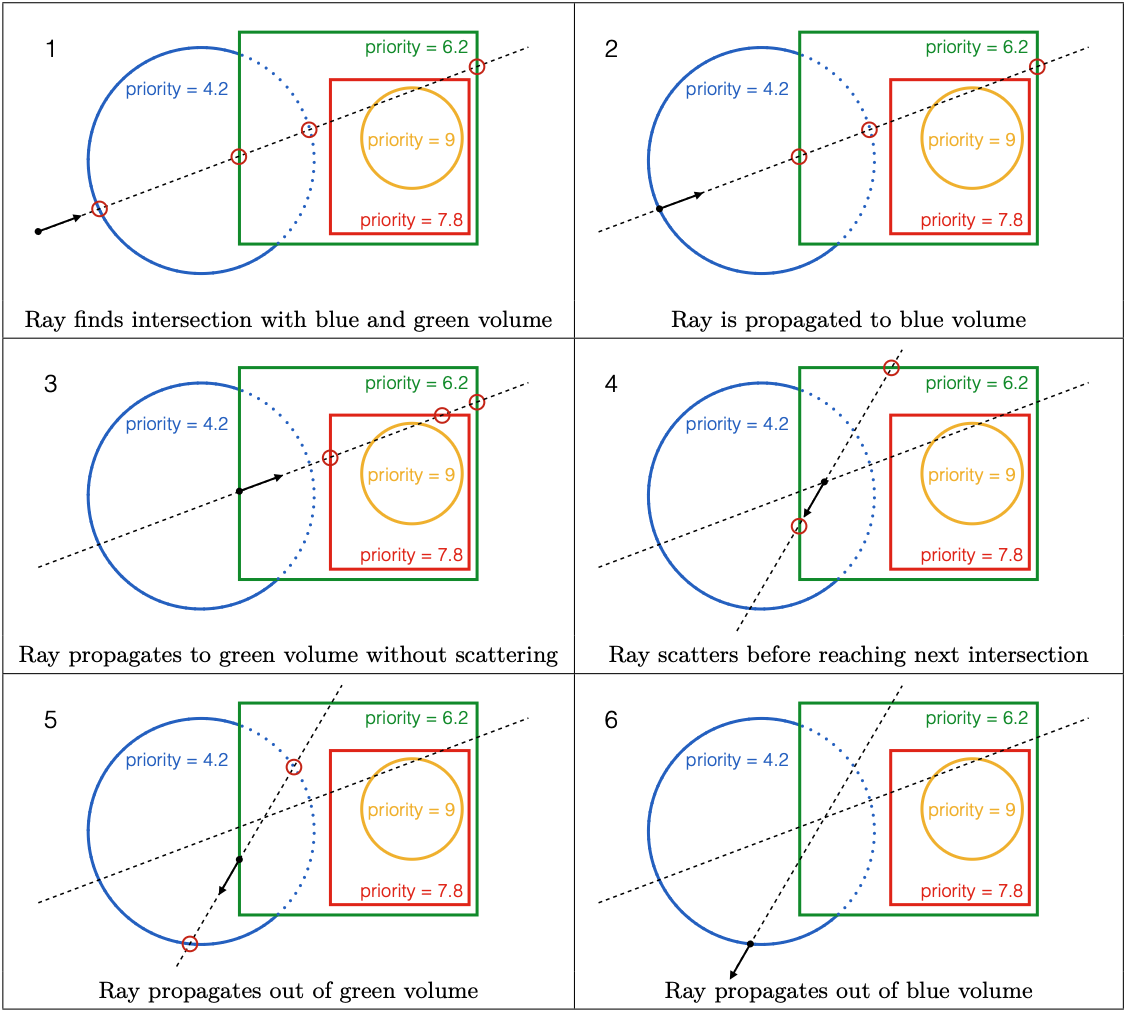
\includegraphics[width=0.9\textwidth]{figures/union_algorithm}
\end{center}
\caption{Illustration of the Union propagation algorithm for a single
  scattering event between two overlapping volumes. Only intersections
  actually relevant given the ray's current volume are calculated at each
  step (the orange volume, never reachable from the ray's actual path
  here, is never tested).}
\label{fig:union-algorithm}
\end{figure}

\subsection{Known limitations}
\label{sec:union-limitations}
\begin{itemize}
\item \textbf{Coincident surfaces.} If two volume boundaries coincide
  exactly, the algorithm cannot reliably determine which volume a ray
  enters. It is safe, and normal, to \emph{overlap} volumes -- but two
  volumes should never be placed so that a face merely touches without any
  overlap or gap; leaving even a micron-scale gap or overlap avoids the
  problem entirely.
\item \textbf{No gravity.} The underlying intersection algorithms are
  linear, so Union volumes propagate in straight lines regardless of any
  gravity setting elsewhere in the instrument (in practice rarely relevant
  for x-ray instruments).
\item \textbf{Feature parity with \MCS.} As noted in
  section~\ref{sec:union-motivation}, loggers, absorption loggers,
  conditionals, surfaces (reflection/refraction) and ray-history tagging
  are not currently available for \MCX's Union components.
\end{itemize}

\section{A complete example}
\label{sec:union-example}

The following excerpt, adapted from the \texttt{PowderCompton\_union}
example instrument (section~\ref{sec:union-further}), combines Compton
scattering in a sphere with powder diffraction in a box:
\begin{lstlisting}
COMPONENT init = Union_init()
AT (0,0,0) ABSOLUTE

COMPONENT compton1 = Compton_xrl_process(density=8.92, atomno=29)
AT (0,0,0) ABSOLUTE

COMPONENT pow2_proc = Powder_process(reflections=refs)
AT (0,0,0) ABSOLUTE

COMPONENT cmpton1 = Union_make_material(
    process_string="compton1", my_absorption=0)
AT (0,0,0) ABSOLUTE

COMPONENT pow2 = Union_make_material(
    process_string="pow2_proc", my_absorption=0)
AT (0,0,0) ABSOLUTE

/* ... source, slits etc. as normal ... */

COMPONENT usphere = Union_sphere(radius=0.25e-3, material_string="cmpton1",
    priority=2)
AT (0,-0.3e-3,0) RELATIVE sample_position

COMPONENT ubox = Union_box(xwidth=1e-3, yheight=0.75e-3, zdepth=0.5e-3,
    material_string="pow2", priority=1)
AT (0,0.8e-3,0) RELATIVE sample_position

COMPONENT master = Union_master()
AT (0,0,0) RELATIVE sample_position

COMPONENT fpi = PSD_monitor_4PI(radius=1.25, nx=101, ny=101, filename="fpi")
AT (0,0,0) RELATIVE sample_position

COMPONENT stop = Union_stop()
AT (0,0,0) ABSOLUTE
\end{lstlisting}
Note the two volumes overlap in neither space nor priority here (a sphere
and a box placed side by side) -- the priority mechanism only matters
where volumes actually share space, as discussed in
section~\ref{sec:union-volumes}.

\section{Further examples}
\label{sec:union-further}

The example instrument library ships Union examples in the
\texttt{Tests\_union} category, including \texttt{PowderCompton\_union}
(the basis for the worked example above, combining Compton and powder
scattering), \texttt{Test\_KN\_Comp\_Rayl\_union} (comparing the
Klein-Nishina, Compton and Rayleigh processes) and \texttt{Geometry\_test}.
See the User Manual's chapter on instrument examples for how to browse
these. A number of the individual component headers, documented in the
Component Manual's Union chapter, contain further short usage examples.

\index{Union|)}
